\documentclass[11pt, letterpaper]{article}  % change to >11 pt if you like, and change article with report
\usepackage[letterpaper, top=3.71cm, bottom=3.20cm, left=2.86cm, right=2.86cm]{geometry}
\usepackage[utf8]{inputenc}
\usepackage{natbib}
\usepackage{amssymb}
\usepackage{graphicx}
\usepackage{color}
\usepackage{chngcntr}
\usepackage{subfig}
\usepackage{float}
\usepackage{hyperref}
\usepackage{url}
\definecolor{bg}{gray}{0.95}
\usepackage{minted}
\usepackage[table, dvipsnames]{xcolor}
\usepackage{mathtools, nccmath}
\usepackage{multirow}
\usepackage{wrapfig}
\usepackage[linesnumbered, ruled, vlined]{algorithm2e}
\usepackage[table, dvipsnames]{xcolor}
\newtheorem{theorem}{Theorem}
\numberwithin{equation}{section}
\counterwithin{figure}{section}
\pagenumbering{gobble}


\title{\vspace{-2cm}\textbf{Computational Health Laboratory project report}}
\author{\textbf{\small{\textit{Dalla Noce Niko, Ristori Alessandro, Zuppolini Andrea}}} \\ % put your full name here
        \small{Master Degree in Computer science.}\\ \small{{n.dallanoce@studenti.unipi.it, a.ristori5@studenti.unipi.it, a.zuppolini@studenti.unipi.it}.} \\  % put your Master Degree here
        \small{Computational Health Laboratory, Academic Year: 2021/2022} \\
        \small{Date: 16/05/2022} \\
       \textbf{\small{\url{https://github.com/nikodallanoce/ComputationalHealthLaboratory}}}
}

\renewcommand\refname{} %remove this line to automatically show the bibliography header

\begin{document}
\nocite{*}  % comment this line to list only the articles you really cite
\date{}
\maketitle
\begin{center}
    
\includegraphics[width=0.3\textwidth]{images/unipi.png} \\
    \vspace{0.5cm}
\end{center}
\begin{abstract}
Starting from one or more genes, extract from interaction databases the genes they interact with. Using the expanded gene set, perform pathway analysis and obtain all disease pathways in which the genes appear. Merge the pathways to obtain a larger graph. Perform further network analysis to extract central biomarkers and communities beyond pathways. Compute a distance between the initial gene set and the various pathways (diseases).
\end{abstract}
\newpage
\tableofcontents
\newpage
\listoffigures
\newpage
\pagenumbering{arabic}
\section{Introduction}\label{sec:introduction}
\subsection{Setting and case study}\label{subsec:settings_case_study}
The Zhu-Tokita-Takenouchi-Kim (ZTTK) syndrome is a recently discovered disease caused by loss of functions in the gene SON \cite{kushary2021zttk}. The heterozygous mutations in this gene is autosomal dominant, with high probability of being inherited.
\vspace{3mm}

The most common feature of the ZTTK are intellectual disability, facial dysmorphism, brain malformation and other features linked to brain and the development of the individual but also ocular, facial and physiological features appears to be linked. There are two main ways to detect ZTTK: Brain imaging and WES (whole exome sequencing). The former is a common methodology and the patient showed many abnormalities in form and shape of the brain, but those characteristics are widely shared with many other neurological diseases. The latter is more precise and guarantees good results in identifying mutations in the gene, being more expensive.
\vspace{3mm}

The difficulties in diagnosis and the poor quantity of data available make the ZTTK a hard disease both to study and identify. Since the only known responsible, up to now, is the SON gene, it becomes tough to circumscribe the set of causes and effects of the ZTTK. In those cases, techniques like geneset augmentation, pathway finding, pathway analysis, clustering and community detection, can really provide powerful tools to the researchers on the field to simplify their analysis and give them relevant statistics helpful to their experimenting.

\subsection{Project roadmap}\label{subsec:project_roadmap}
This project report follows the roadmap we present here:
\begin{enumerate}
    \item \textbf{Geneset-expansion}, starting from the gene SON and its interactions, we have expanded our set using $1^{st}$ and $2^{nd}$ order neighbourhood, querying the BioGRID \cite{biogrid} database. The network was now big enough to find other pathways;
    \item \textbf{Pathway enrichment}, using the GSEApy \footnote{https://github.com/zqfang/GSEApy} package we have performed pathway enrichment with the data in the DisGeNET \cite{disgenet} to  associate the genes with the disease pathways they contribute to;
    \item\textbf{Network analysis}, after building the network, two metrics have been deployed to analyze the diseases on it, such as the distance among the pathway components, the largest pathway component size. Afterwards, we have used the node's degree inside the network to extract the most significant biomarkers;
    \item \textbf{Community analysis}, as first step we decided on using the Louvain method for detecting the communities, we found between $8-11$ communities starting from the graph we have built, weighting the edges using the number of shared diseases between the couples of nodes. Then we compared the pathways in the community we have found for the SON gene with the known relevant effect of the ZTTK syndrom, along with many other metrics.
\end{enumerate}
\section{Geneset Expansion}\label{sec:geneset_expansion}
As we said in \autoref{sec:introduction}, the only known responsible of the ZTTK disease, up to know, is the SON gene, even though it is a well known gene that contributes to the RNA splicing and the overall cell cycle. In order to study possible concurrent factor to the syndrome we have first enlarged the geneset under our focus (which we retrieved into a csv format from BioGRID \cite{biogrid} and cleaned by hand) by looking at all of the genes that interact with SON and, iteratively, also the second order neighbourhood. The request for the $1^{st}$ order neighbourhood retrieved 146 proteins and their (eventual) mutual interactions as we can see in \autoref{fig:starting_interactions} \subref{subfig:first_order_interactions}, the second request enlarged our network to $12863$ nodes.
\begin{figure}[H]
    \centering
    \subfloat[The $146$ starting interactions \label{subfig:son_interactions}]{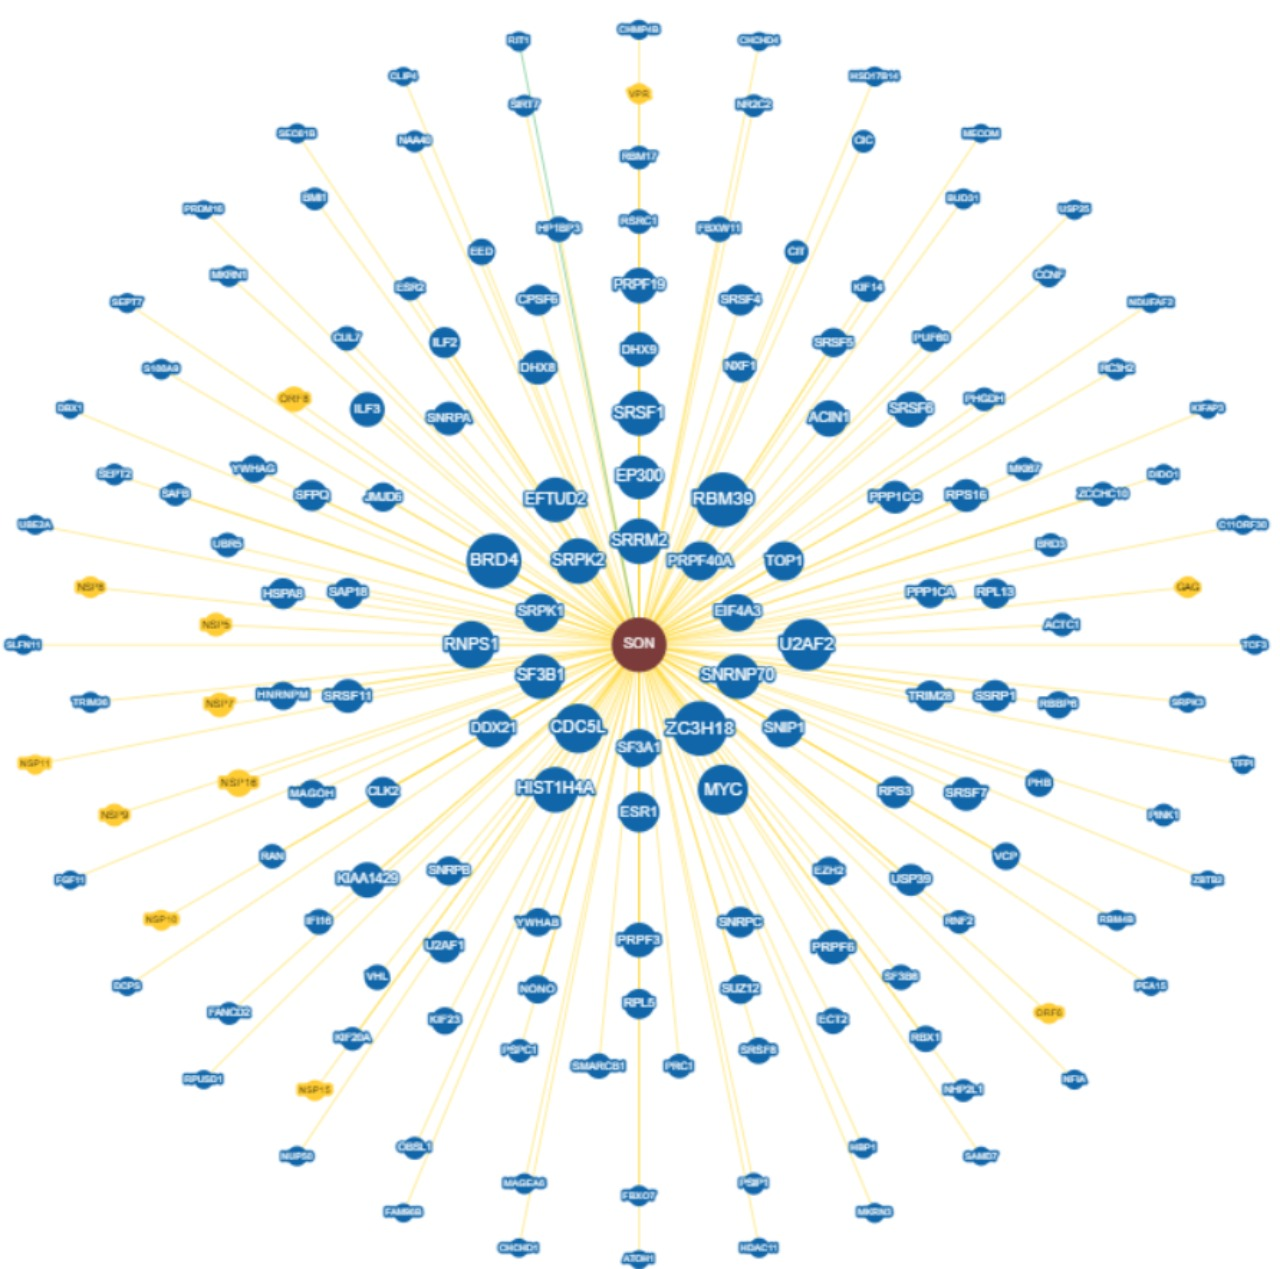
\includegraphics[width=0.5\linewidth]{images/geneset_starting_interactions.jpg}}
    \subfloat[The interactions at the first order \label{subfig:first_order_interactions}]{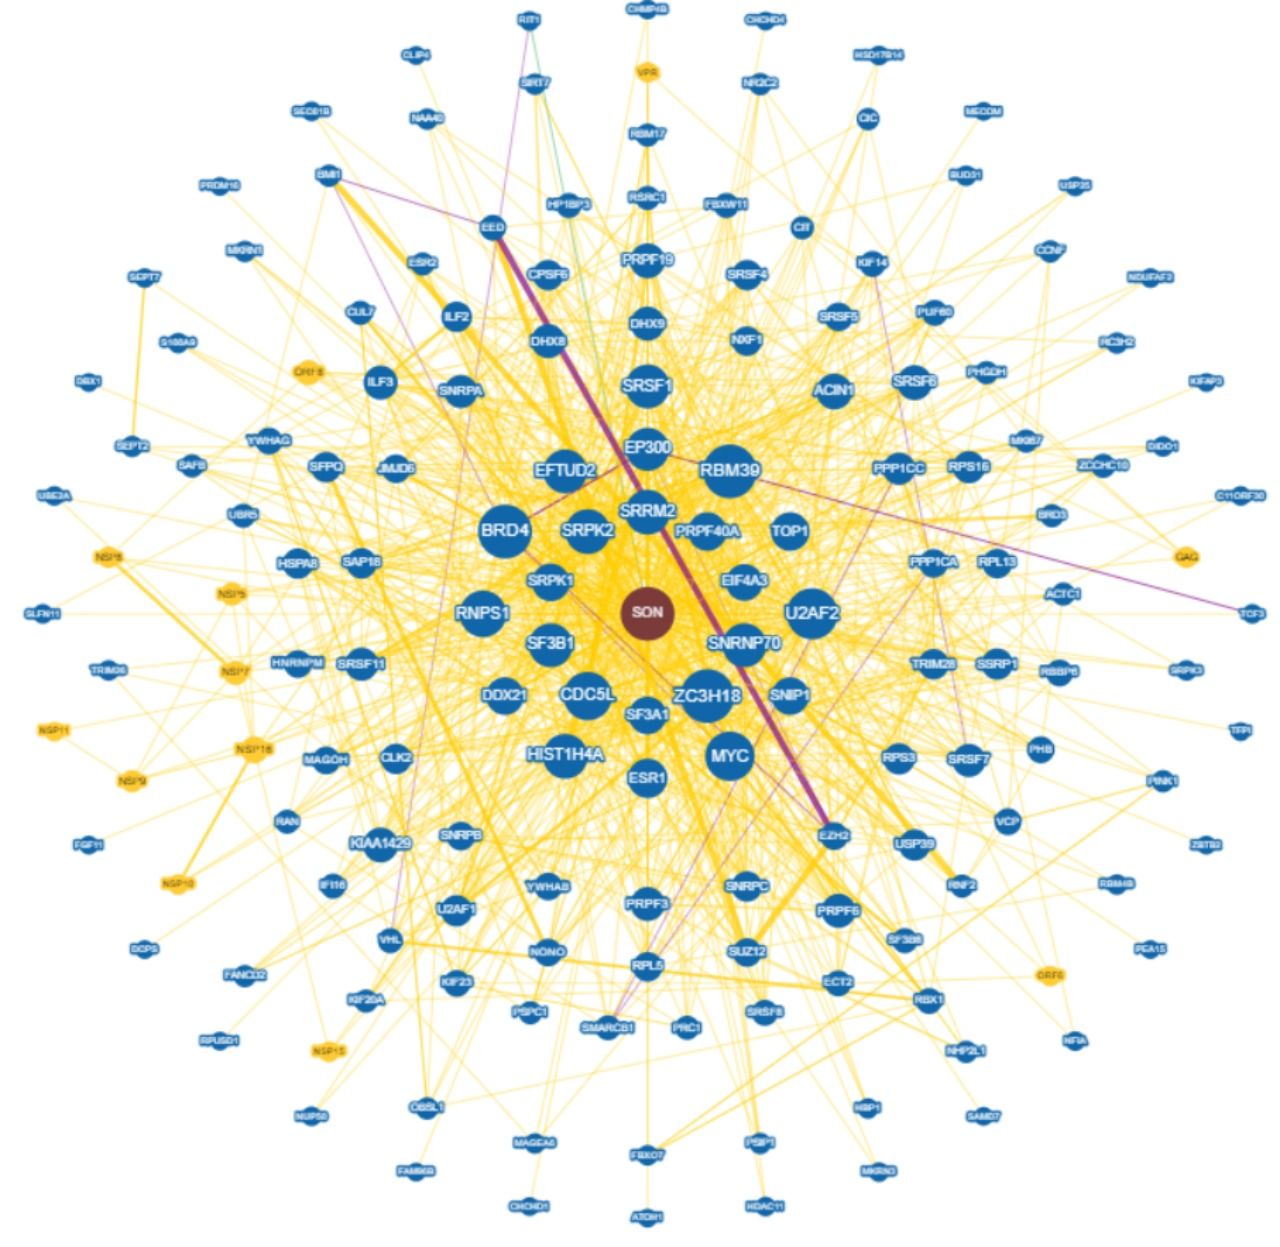
\includegraphics[width=0.5\linewidth]{images/geneset_first_order.jpg}}
    \caption{Starting interactions from the SON gene and all the first order interactions.}
    \label{fig:starting_interactions}
\end{figure}
All the information retrieved has been post-processed:
\begin{itemize}
    \item All the genes have been upper cased, the BioGRID dataset is mantained by its users, so we needed to uniform them;
    \item All the duplicated interactions were removed, there were $25281$ of such interactions and we did not them since our graph is not directed;
    \item All the self loops were removed, we are not interested in a protein interaction with itself.
\end{itemize}
As we can see in \autoref{fig:starting_interactions}, the shape of the network is well-defined, SON is at the center of the interactions and all of the nodes are distributed around it at a distance path of $2$, while two generic proteins can have a maximum distance of $4$. This graph is the starting point of our analysis, we have now a significant amount of data to perform a satisfying pathway enrichment 
\section{Pathway Enrichment}\label{sec:pathway_enrichment}
In this section, we start from the gene set obtained in \autoref{sec:geneset_expansion} to find all the disease pathways linked to it, to accomplish that we have used GSEApy, a python package that performs pathway enrichment from many sources. At first we tried with the KEGG and Reactome human datasets with no success since we would have to manually remove all those pathways not related to any disease and there was no way to filter them out, then we found the DisGeNET dataset \cite{disgenet}, which satisfied our needs.
\vspace{3mm}

Passing to the GSEApy \textit{enrichr} method all the nodes in our graph, it performed pathway enrichment on our behalf, then, we filtered the disease pathways by keeping those having a p-value lower than $0.1$, totalling $589$ pathways which will be used during our future network and community analysis.
\vspace{3mm}

An example of disease pathway is in \autoref{fig:example_disease_pathway}, a big number of proteins are do not interact between each other, this is totally normal given the size of our graph and the fact that we centered it around a specific gene and limited it at the second order.
\begin{figure}[H]
    \centering
    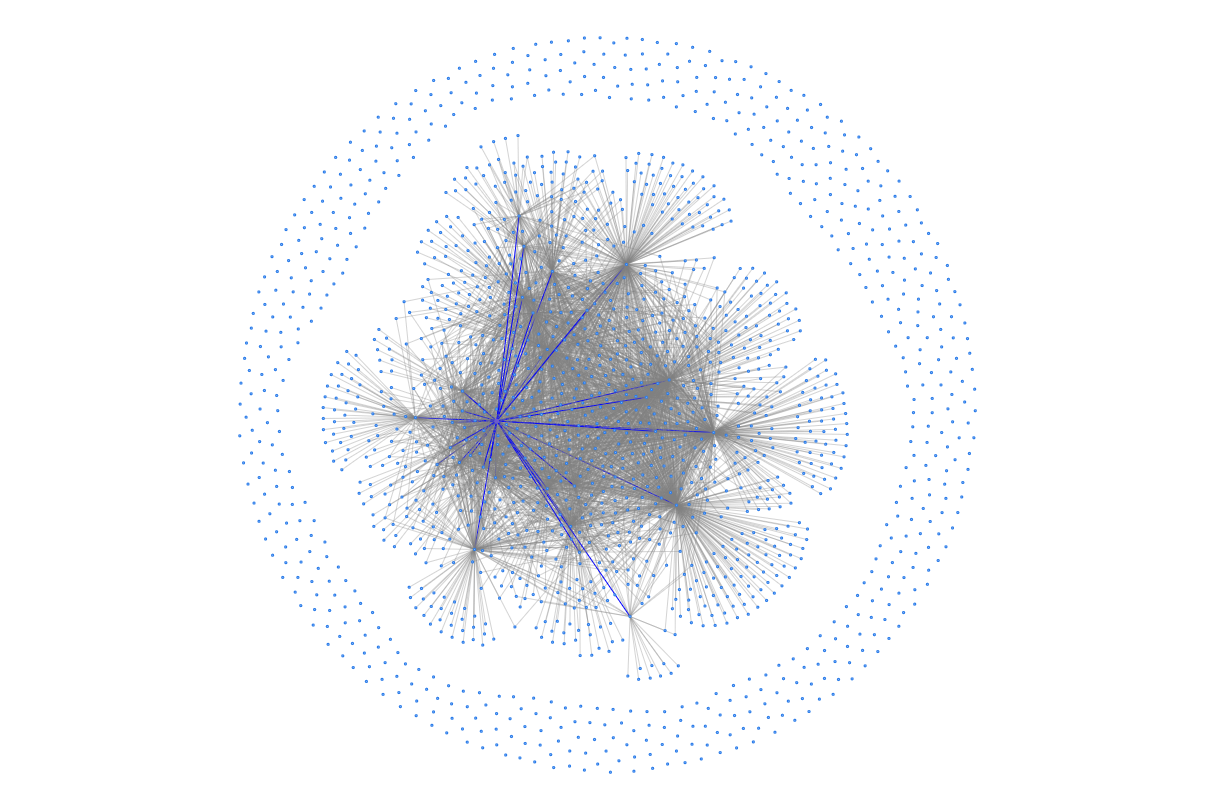
\includegraphics[width=1\linewidth]{images/plots/disease_pathway_graph.png}
    \caption{A disease pathway with the SON gene and its interactions highlighted in blue.}
    \label{fig:example_disease_pathway}
\end{figure}

The GSEApy package, no matter the dataset, always returns a dataframe with following columns (\autoref{fig:disease_pathways} shows such dataframe):
\begin{itemize}
    \item \textbf{Term}, the disease pathway name.
    \item \textbf{Overlap}, the ratio of the disease's genes that are in our graph over the entire number of its gene, the former is more useful than the latter for our analysis.
    \item \textbf{P-value}, how much the result is trustable.
    \item \textbf{Adjusted P-value}, the P-value obtained over all the significant tests.
    \item \textbf{Genes}, a string formed by all the genes of our graph that belong to the pathway, they are comma separated.
\end{itemize}
\begin{figure}[H]
    \centering
    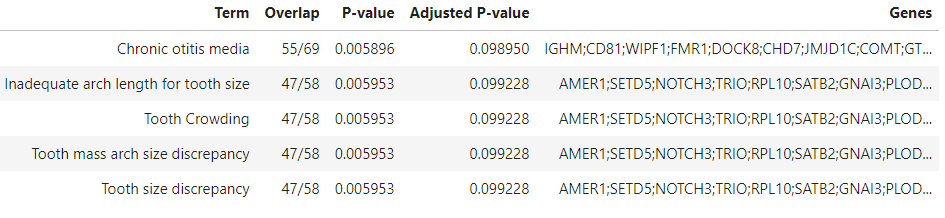
\includegraphics[width=1\linewidth]{images/disease_pathways.png}
    \caption{An example of disease pathways retrieved by using the GSEApy package.}
    \label{fig:disease_pathways}
\end{figure}
Since working with the dataframe genes attribute was not so convenient due to it being a string which we would have to split each time we would have to work with the pathways, we decided to build a dict indexed by the disease's indexes (the first column of the dataframe as seen in \autoref{fig:disease_pathways}) and using the term as the "name" and the splitted genes as a list attribute.
\section{Network Analysis}\label{sec:network_analysis}
\subsection{Building the protein-to-protein graph}\label{subsec:protein_to_protein_graph}
Starting from the interaction dataset built after the geneset expansion (as we have seen in \autoref{sec:geneset_expansion}) we developed our protein-to-protein network thanks to the networkx\footnote{https://github.com/networkx/networkx} python package. First we inserted the nodes into the graph and named them with the protein they represent, and, at the same time we "colored" them with the disease pathways they belong to. Then, we created the edges from the interaction dataset and we weighted them based on the number of shared diseases (the ones retrieved during the pathway enrichment explained in \autoref{sec:pathway_enrichment}) between couple of nodes.
\vspace{3mm}

We noticed that a relevant number of nodes/proteins does not belong to any disease, more precisely $5101$ of the $13010$ proteins. Since we did not want to end with possibly a non-connected graph, we decided to keep them. The same can also be seen for the edges, since we have observed that $45000$ of them had no shared diseases between the couple of nodes they connect, but the same reasoning we did for the nodes stands for them, so we kept them too. \autoref{fig:nodes_edges_no_disease} shows the how we computed such nodes and edges after building our protein-to-protein graph.
\begin{figure}[H]
    \centering
    \subfloat[Nodes with no color/disease]{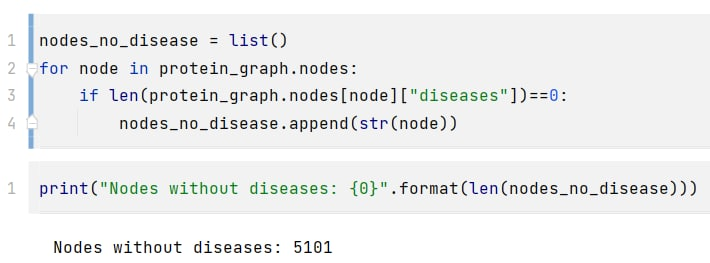
\includegraphics[width=0.5\linewidth]{images/nodes_no_diseases.jpg}}
    \subfloat[Edges with no weight/disease]{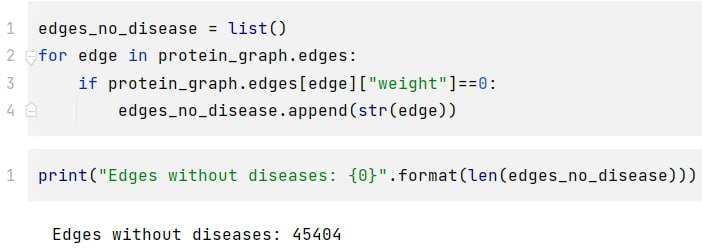
\includegraphics[width=0.5\linewidth]{images/edges_no_diseases.jpg}}
    \caption{Jupyter cells that compute the number of nodes and edges that do not belong to any disease pathway.}
    \label{fig:nodes_edges_no_disease}
\end{figure}

\subsection{Disease network metrics}\label{subsec:disease_metrics}
Once we built the protein-to-protein graph (we talked about it in \autoref{subsec:protein_to_protein_graph}) we computed some of the metrics proposed by Agrawal et al. \cite{agrawal2018} to have a better overview on the effect of each disease pathway on our newly built graph.
\paragraph{Size of largest pathway component} \textit{Fraction of disease proteins that lie in the disease's largest pathway component (i.e., the relative size of the largest connected component (LCC) of the disease)} \cite{agrawal2018}. It indicates how prevalent is the biggest component of genes inside a disease pathway and, therefore, how its genes are connected between them.
\paragraph{Distance of pathway components} \textit{For each pair of pathway components, we calculate the average shortest path length between each set of proteins, and then, the average of this is taken over all pairs of the components} \cite{agrawal2018}. Even though this metric tells us how distant are a disease's genes and, therefore, how long is the path between them, it is not valuable in our case since, as we explained at the end of \autoref{sec:geneset_expansion}, our graph is centered around the SON gene and, for that reason, the maximum distance of each node from one another is $4$.

\subsection{Biomarkers identification}\label{subsec:biomarkers}
A main issue, not the hardest but for sure the most annoying and tedious one, was related to plotting the graph, which had too many nodes and interactions to be properly drawn. Moreover, we were interested in knowing which were the biomarkers, the "central" nodes of our graph, the ones that have more "impact" on its connectivity. Solving the latter would have also made the plotting far easier, so we it was a logical step at the end of our network analysis.
\vspace{3mm}

By using the centrality algorithm based on the nodes' degree from the networkx package, we made a method that retrieves a user-specified number of biomarkers plus one protein of their choice (in our case the SON gene). \autoref{fig:biomarkers} shows the $30$ biomarkers identified whose centrality is the ratio between the node degree over the entire number of nodes that compose the protein-to-protein graph.
\begin{figure}[H]
    \centering
    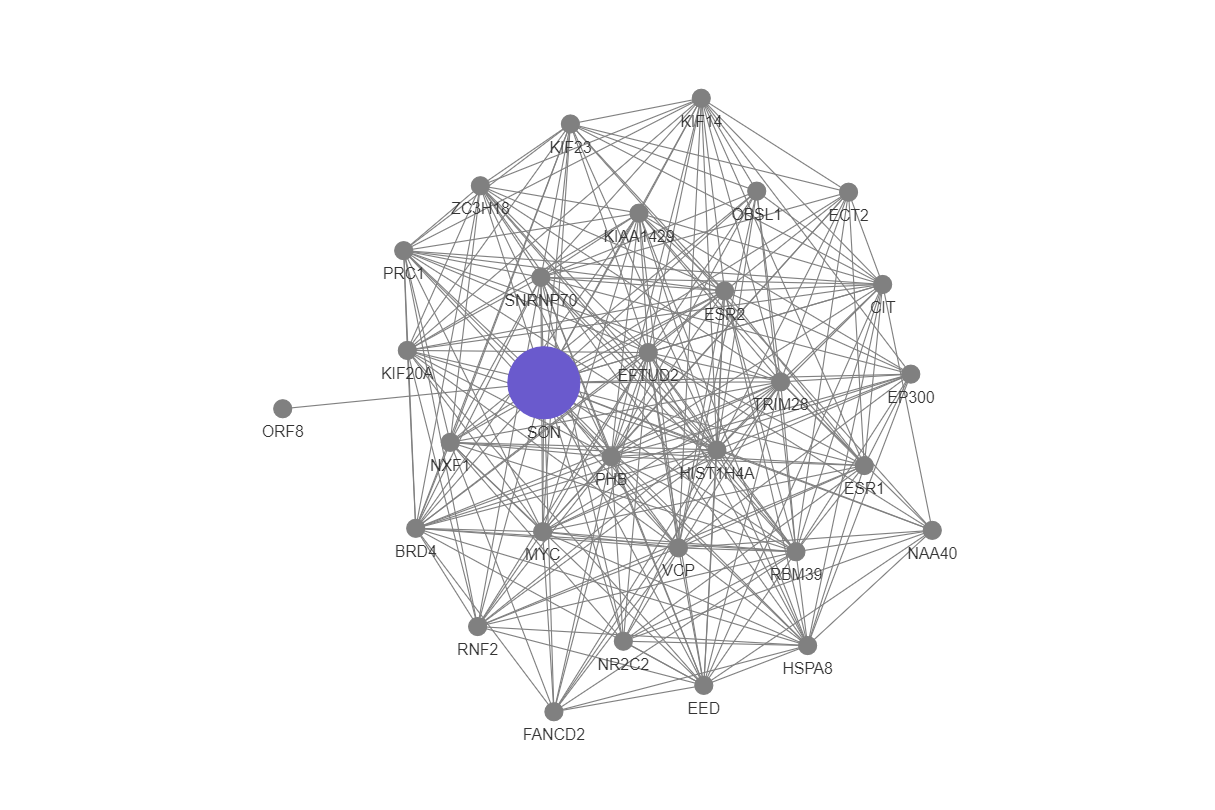
\includegraphics[width=1\linewidth]{images/plots/plot_biomarkers.png}
    \caption{Biomarkers with the SON gene highlighted.}
    \label{fig:biomarkers}
\end{figure}
\section{Community Analysis}\label{sec:community_analysis}
\subsection{Community detection}\label{subsec:community_detection}
At this point, a protein graph is available, weighted using the shared disease (\autoref{subsec:protein_to_protein_graph}), that could be helpful to reveal potential clusters of nodes with similar features. However, since our goal is to find non trivial relationships of genes and pathways with the SON gene, the most interesting features in our study case are the hidden features. Namely, the ones which are not directly available but have to be extracted working with the network, using methods like community detection.
\vspace{3mm}

Since our network is quite large in terms of both nodes and especially edges, we have decided to use the \textit{Louvain method} for community detection having time complexity $\mathcal{O}(n \cdot \log{n})$, with $n$ being the number of nodes. The Louvain method is a greedy algorithm that optimizes the network modularity \eqref{eq:modularity}:
\begin{equation}
    Q = \frac{1}{2m} \sum_{i,j}\left[ A_{ij} - \frac{k_i k_j}{2m} \right] \delta(c_i, c_j)
    \label{eq:modularity}
\end{equation}
This approach distinguishes group of nodes with high density of connections and delimits the community whenever there is a drop of density in the number of edges. The algorithm stops whenever a local maximum of network modularity is reached, therefore different execution can lead to different detection of the communities.
\vspace{3mm}

The algorithm gives back around $6900$ different communities, but most of those are made of singletons of only one gene. Performing a cross-check with the initial protein-graph we have noticed that most of those single-gene communities are involved in a minimal number of pathways, in average $2$ as seen in \autoref{fig:mean_diseases_nodes_communities} \subref{subfig:mean_diseases_community}, or are not involved in any pathways at all. Usually, running the algorithm, only between $[8-11]$ communities have a significant number of genes with around $680$ genes per community (\autoref{fig:mean_diseases_nodes_communities} \subref{subfig:mean_community_size}), while the remaining ones, the singletons, are sort of outliers, therefore we have decided to leave them out. Up to now, the remaining communities cover more than $6100$ genes and we have implemented many methods to highlight their characteristics.
\begin{figure}[H]
    \centering
    \subfloat[Average singleton community size \label{subfig:mean_diseases_community}]{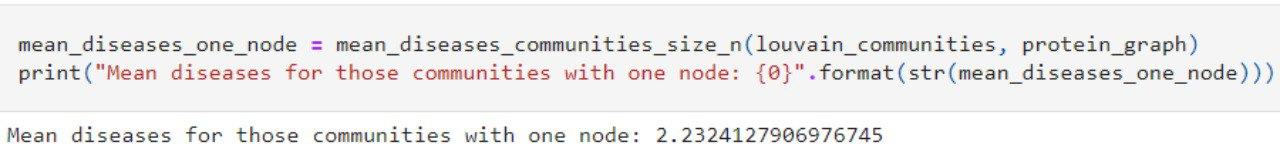
\includegraphics[width=1\linewidth]{images/singletons_mean_size.jpg}}\\
    \subfloat[Average community size \label{subfig:mean_community_size}]{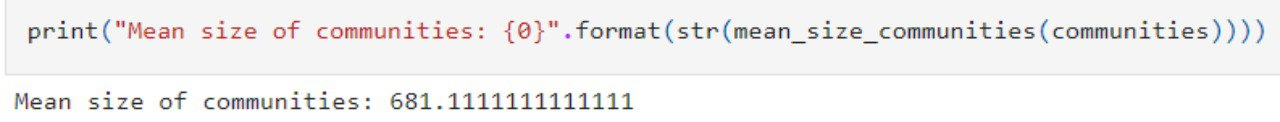
\includegraphics[width=1\linewidth]{images/community_mean_size.jpg}}
    \caption{Number of diseases for single-gene communities and mean size of kept communities.}
    \label{fig:mean_diseases_nodes_communities}
\end{figure}
Such communities were then plotted with the pyvis package\footnote{https://github.com/WestHealth/pyvis} by assigning different colors to better visualize them as we can see from \autoref{fig:communities}, we highlighted the SON gene by giving it a bigger size than all the other nodes in the graph. More graphs will be shown in \autoref{sec:results} to better illustrate the results.
\begin{figure}[H]
    \centering
    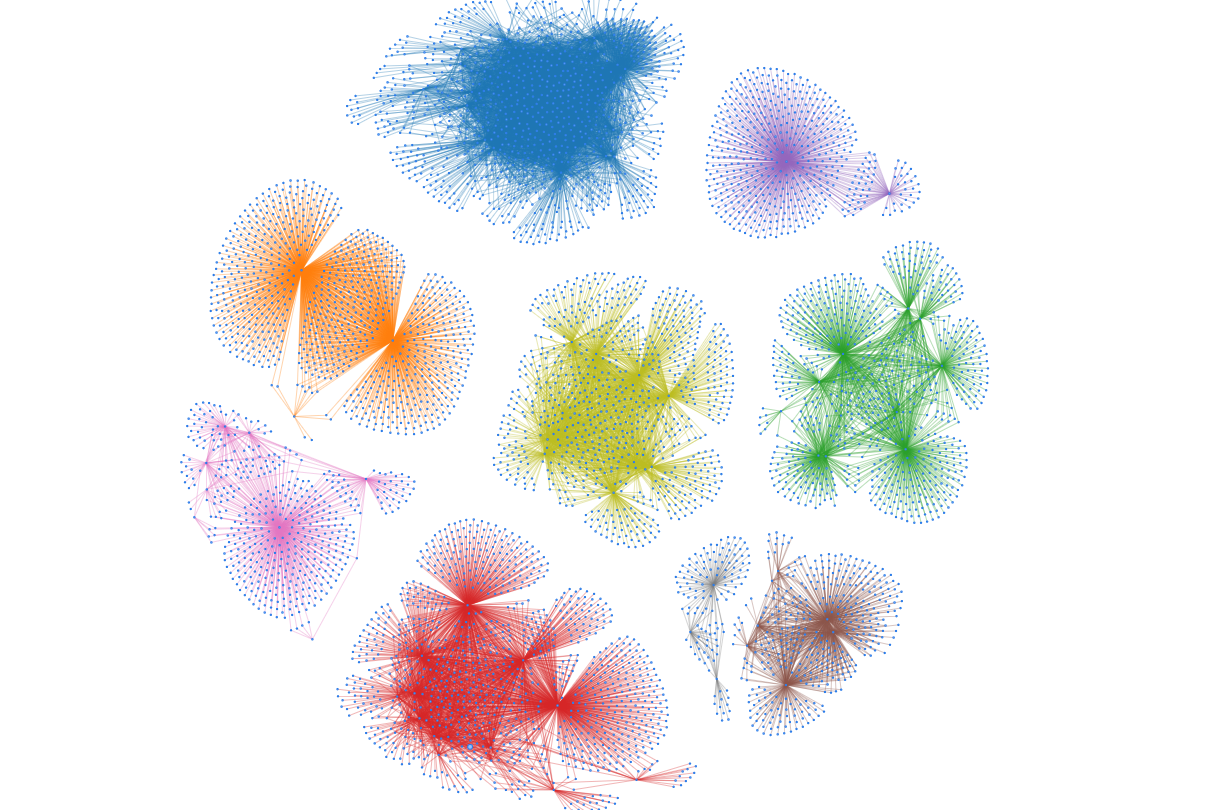
\includegraphics[width=0.9\linewidth]{images/plots/communities.png}
    \caption{Communities after the pruning.}
    \label{fig:communities}
\end{figure}

\subsection{Community evaluation}\label{subsec:community_evaluation}
In this section there will be the evaluation of the communities, which, in our example, there are $9$ of them (\autoref{fig:communities}). Every community contains a number of nodes which is involved in many different disease pathways and, to evaluate the goodness of the various clusters, we have implemented several metrics:
\begin{itemize}
    \item \textbf{Ratio disease}, measuring the ratio between the genes of the given community which participate to a disease pathway over the whole size of that pathway. This metric is particularly useful to avoid that the largest pathways are always the major contributors of the community. For example the "Malignant neoplasm of breast", which has around 3400 genes, without this metric would be the most relevant disease in almost every community. Scaling it with its size, gives a better perspective of its actual contribution in the interval $(0,1]$.
    \begin{equation}
        R_d = \frac{n_c}{n_d}
        \label{eq:ratio_disease}
    \end{equation}
    \item \textbf{Ratio community}, again a ratio, this time between the number of genes in a given pathway over the size of the community.This other metric puts in relation the contribution of every pathway in a given community with the community size, rewarding pathways with a lot of contribution in the community and has value in the interval $(0,1]$, this metrics solves the problem with small pathways entirely contained in the same community.
    \begin{equation}
        R_c = \frac{n_c}{|V_c|}
    \end{equation}
    \item \textbf{Relevance}, represents the best of both worlds. It combines the absolute contribution of the pathway with the community size, and is obtained multiplying the previous 2 metrics. It has, again, values in the interval $(0,1]$. 
    \begin{equation}
        Relevance = R_d \times R_c
    \end{equation}
\end{itemize}
\begin{figure}[H]
    \centering
    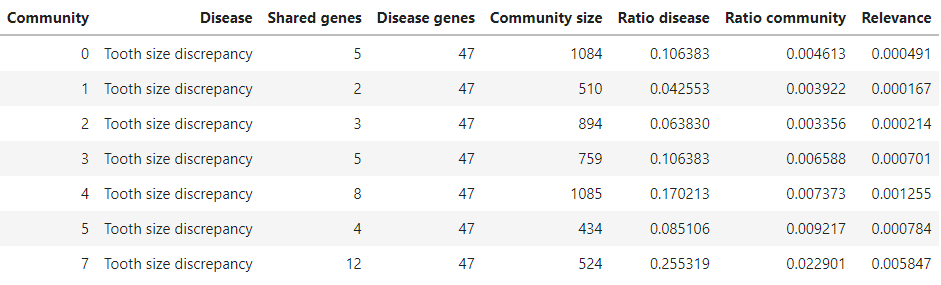
\includegraphics[width=1\linewidth]{images/disease_community_metrics.png}
    \caption{The community-disease dataframe with the computed metrics, we choose a disease as an example.}
    \label{fig:disease_community_metrics}
\end{figure}
By taking into account the computed metrics we can also determine the distance of every community to all the other ones. Since the distance is based on disease-related metrics, it also represents a similarity value between the communities.For our purpose this metric is not relevant since we needed to focus only on the SON community, but it could be useful for future improvement of an hypothetical pathway analysis package.
\begin{figure}[H]
    \centering
    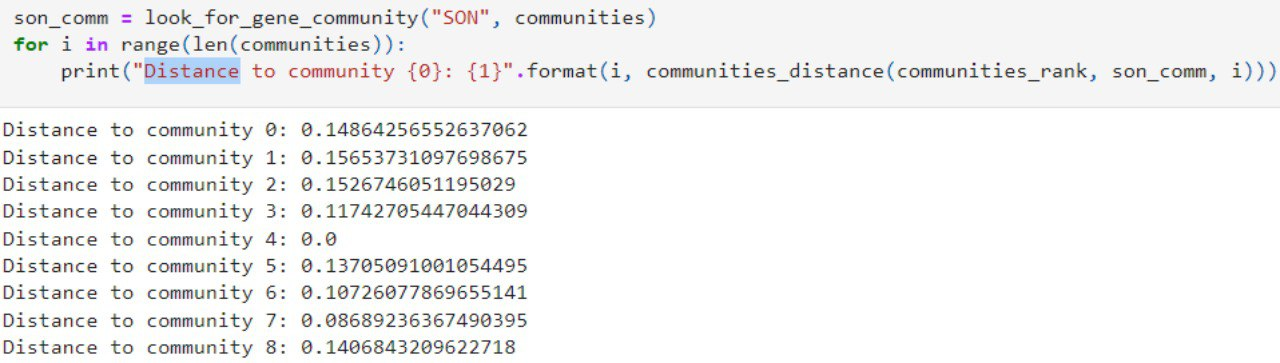
\includegraphics[width=0.8\linewidth]{images/distance_communities.jpg}
    \caption{Distance between the SON gene's community towards the other ones, the lower the value the better.}
    \label{fig:distance_communities}
\end{figure}
\section{Results}\label{sec:results}
In this section we show the results of the community analysis performed in the SON gene's community by applying the metrics presented before, in \autoref{subsec:community_evaluation}.

\subsection{Relevant diseases in SON community}\label{subsec:relevant_diseases}
In \autoref{fig:diseases_son_community} we show the top 10 most relevant diseases inside the SON community:
\begin{figure}[H]
    \centering
    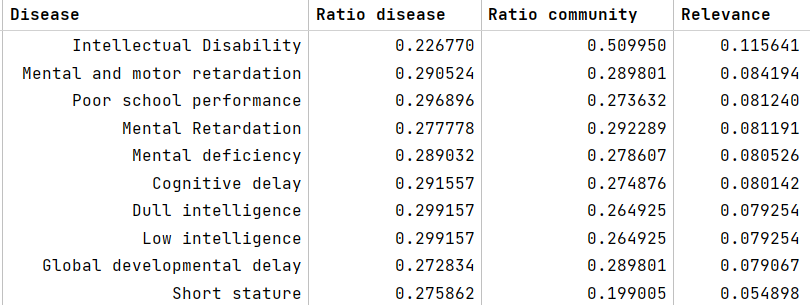
\includegraphics[width=0.9\linewidth]{images/top20_diseases_connected.png}
    \caption{Diseases found in the SON community ordered by Relevance}
    \label{fig:diseases_son_community}
\end{figure}
Those results seems to be coherent with the state-of-the-art knowledge of the ZTTK syndrome, since most of the diseases presented in \autoref{fig:diseases_son_community} are related to neurological pathologies or cognitive difficulties, coherently with the ZTTK collateral aspects. Especially for \textit{Intellectual Disability}, encountered in $100\%$ of the ZTTK diagnoses, our results have evidenced the strong link between the two pathologies. Also, as another example, for the case of \textit{global development delay} most of the patients studied in the ZTTK paper have presented such disease.
\vspace{3mm}

With respect to all the other diseases, their relation with SON should be experimentally verified even though, apparently, they seem to align, more or less, with all the others.
\vspace{3mm}

Those results in \autoref{fig:diseases_son_community} are ordered in terms of Relevance, because of the unbalancing that could be caused by the other two metrics as discussed in \autoref{subsec:community_evaluation}: 
\begin{itemize}
    \item if we sort the rows using the "Ratio disease" we are rewarding bigger disease pathways such as \textit{Malignant breast carcinoma}, and penalizing smaller pathologies even if their overall contribution is bigger.
    \item On the other hand, sorting by "Ratio community" would only emphasize how much the disease contributes to a community without considering its pathway size, thus favoring those small disease contained entirely in a community.
\end{itemize}
 
\subsection{Diseases with SON in their pathways}\label{subsec:diseases_son}
As seen in \autoref{subsec:relevant_diseases}, most of the relevant pathologies inside SON community are well-known effects of the syndrome under inspection, now we need to focus on the disease pathways in which SON belongs to and plot them in order to confirm what we have seen until now.
\vspace{3mm}

Let's visualize directly on \autoref{fig:intellectual_disability_SON}, \autoref{fig:undergrowth_SON} and \autoref{fig:strabismus_SON} the results of our analysis, evidencing the three disease pathways inside SON gene's community. Just to point out a needed observation, the diamond nodes represents genes that belong to such pathway and we colored in orange the edges that connect them, meanwhile the SON gene was highlighted in blue to better distinguish it from the other proteins.
\begin{figure}[H]
    \centering
    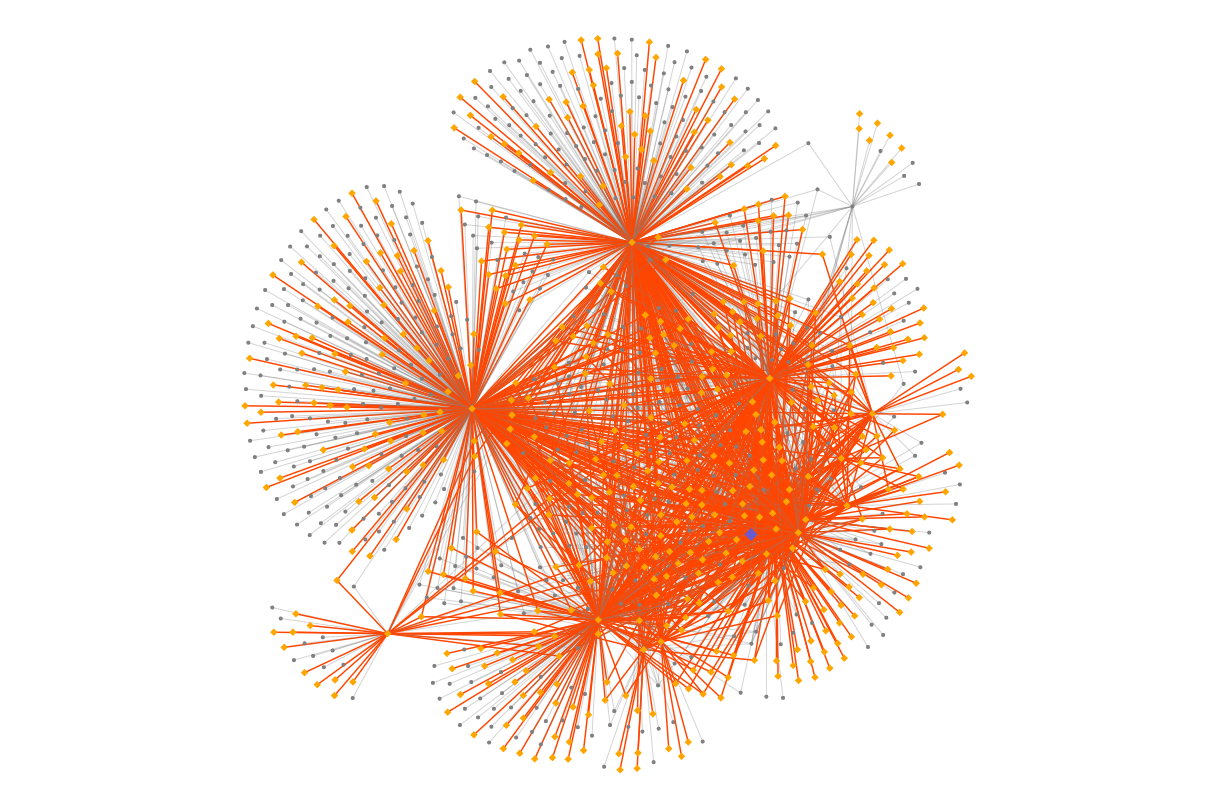
\includegraphics[width=1\linewidth]{images/plots/intellectual_disability_SON.png}
    \caption{Intellectual disability disease pathway within the SON community.}
    \label{fig:intellectual_disability_SON}
\end{figure}
Inside the community there are, more or less, $700$ nodes and it can also be noticed that the pathways are well integrated inside the community, as seen for \textit{Intellectual disability} in \autoref{fig:intellectual_disability_SON}, since its genes are connected to many hub nodes, but this was expected as that disease has the highest "Relevance" value.
\vspace{3mm}

Let's now plot in \autoref{fig:undergrowth_SON} and \autoref{fig:strabismus_SON} two more disease pathways that have SON as their gene but do not have a big "Relevance" value as the previous one.
\begin{figure}[H]
    \centering
    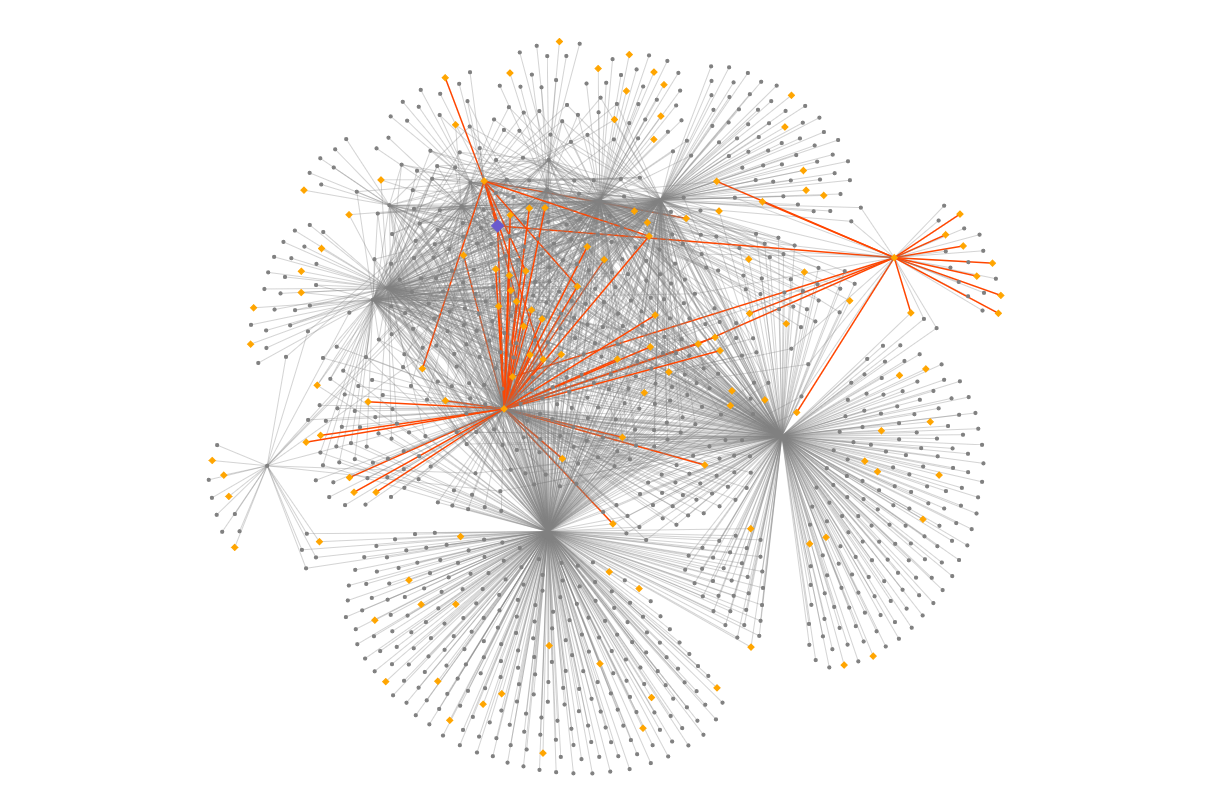
\includegraphics[width=0.8\linewidth]{images/plots/undergrowth_SON.png}
    \caption{Undergrowth disease pathway within the SON community.}
    \label{fig:undergrowth_SON}
\end{figure}

\begin{figure}[H]
    \centering
    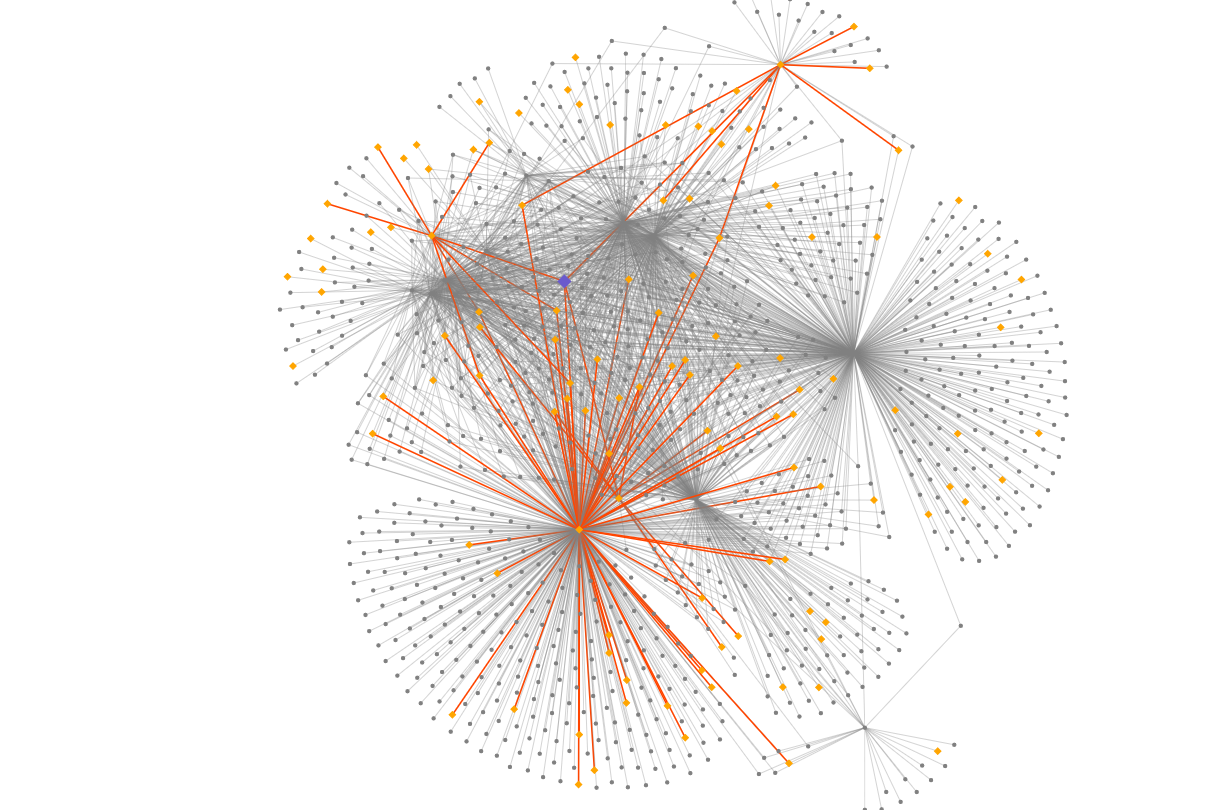
\includegraphics[width=0.8\linewidth]{images/plots/strabismus_SON.png}
    \caption{Strabismus disease pathway within the SON community.}
    \label{fig:strabismus_SON}
\end{figure}

\subsection{Diseases without SON in their pathways}\label{subsec:diseases_no_son}
To investigate potential undiscovered correlations between genes in the community and the SON gene, we will now try to explore the diseases which do not contain the latter but manifest a strong interaction in its community. In particular, it is very useful plotting these disease pathways in order to see which of them interact with SON. In \autoref{fig:top_20_diseases_disconnected} we show the collected top 20 diseases that don't have the SON gene in their pathway, ordered by the "Relevance" metric.
\begin{figure}[H]
    \centering
    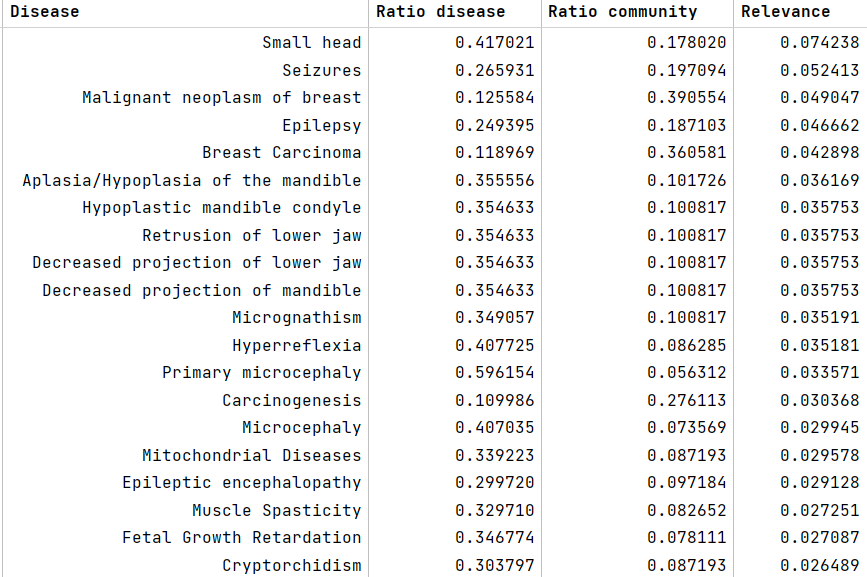
\includegraphics[width=0.8\linewidth]{images/top20_diseases_disconnected.png}
    \caption{The top 20 diseases disconnected from SON, but in its same community.}
    \label{fig:top_20_diseases_disconnected}
\end{figure}
Beware, many of the disease we have found, do not have a known relation with ZTTK, hence their link should be experimentally verified. For the \textit{Epilepsy} disease this could be a significant result, since it has been encountered in some of the patients with ZTTK, and those results are a good signal indicating a potential relation. Even if the SON gene is not present in that pathway, at this point, it is reasonable to say that there could be a correlation and hence ZTTK patients could benefit of some of the knowledge the medical community has on epilepsy.
\vspace{3mm}

Some of the rows in \autoref{fig:top_20_diseases_disconnected} present widely studied pathologies such as various types of cancers, but their presence, as already mentioned many times (\autoref{subsec:community_evaluation}), can also derive from the influence that such big pathways have inside strict communities, even though the "Relevance" metric has a mitigation effect on it. Moreover, from the literature, we recall that there is not any proof of correlation between the ZTTK and cancer.
\vspace{3mm}

Furthermore we present some plots (\autoref{fig:small_head_NO_SON}, \autoref{fig:epilepsy_NO_SON} and \autoref{fig:hyperreflexia_NO_SON}) to evidence our results with diseases that do not have SON in their pathways but that could correlated.
\begin{figure}[H]
    \centering
    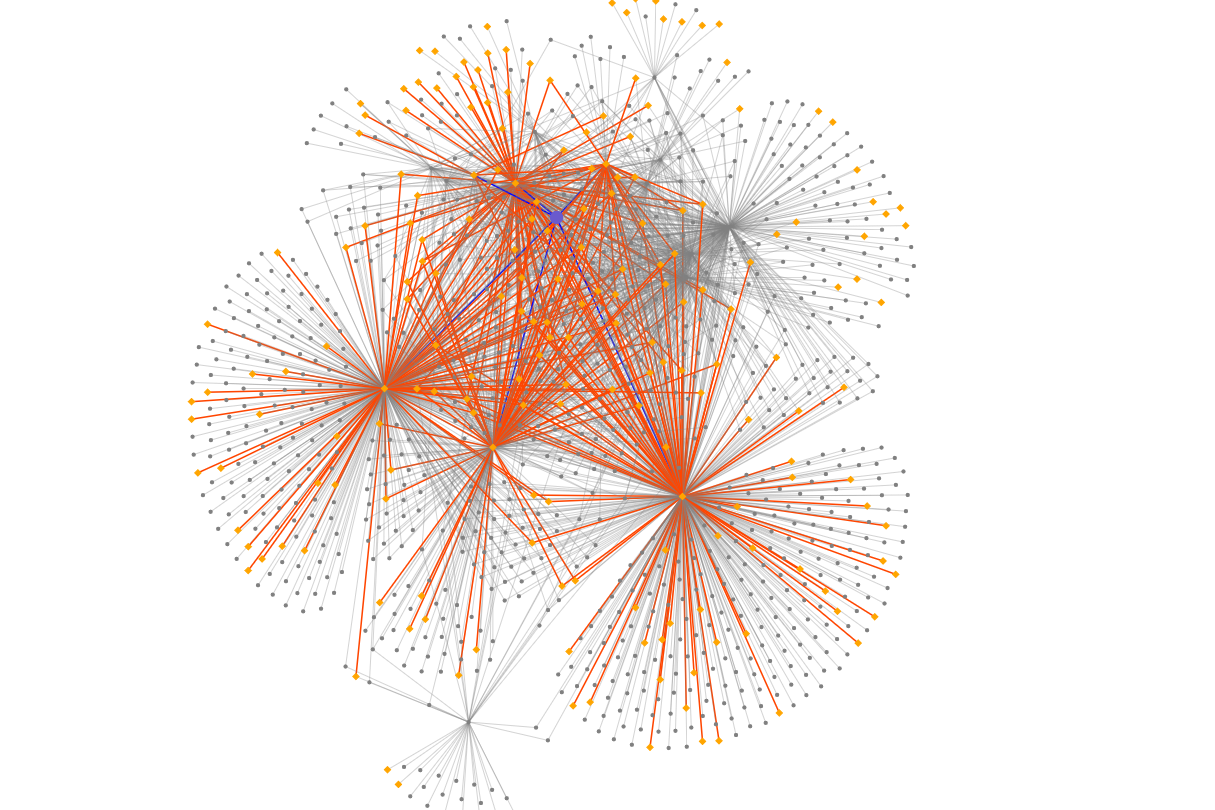
\includegraphics[width=0.8\linewidth]{images/plots/small_head_NO_SON.png}
    \caption{Small head disease pathway within the SON community. Blue edges highlights the interaction between the SON gene and the genes inside the pathway.}
    \label{fig:small_head_NO_SON}
\end{figure}

\begin{figure}[H]
    \centering
    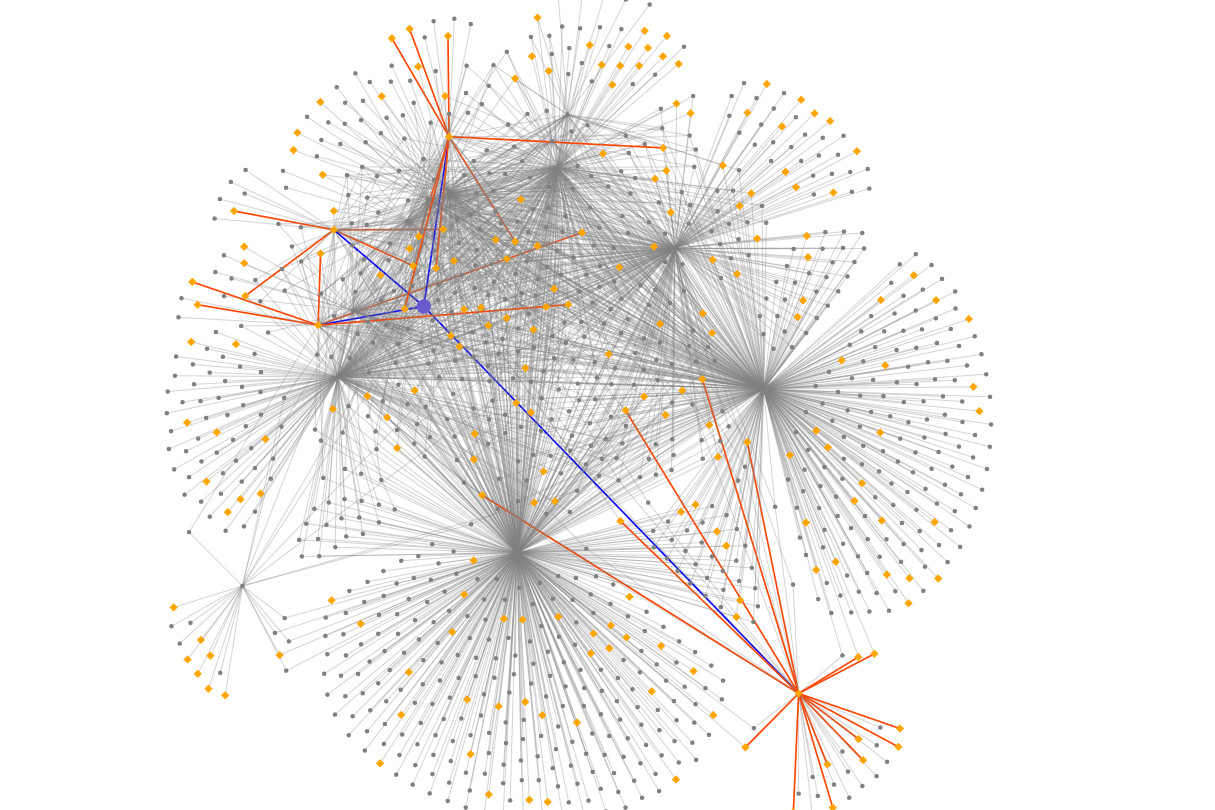
\includegraphics[width=0.8\linewidth]{images/plots/epilepsy_NO_SON.png}
    \caption{Epilepsy disease pathway within the SON community. Blue edges highlights the interaction between the SON gene and the genes inside the pathway.}
    \label{fig:epilepsy_NO_SON}
\end{figure}

\begin{figure}[H]
    \centering
    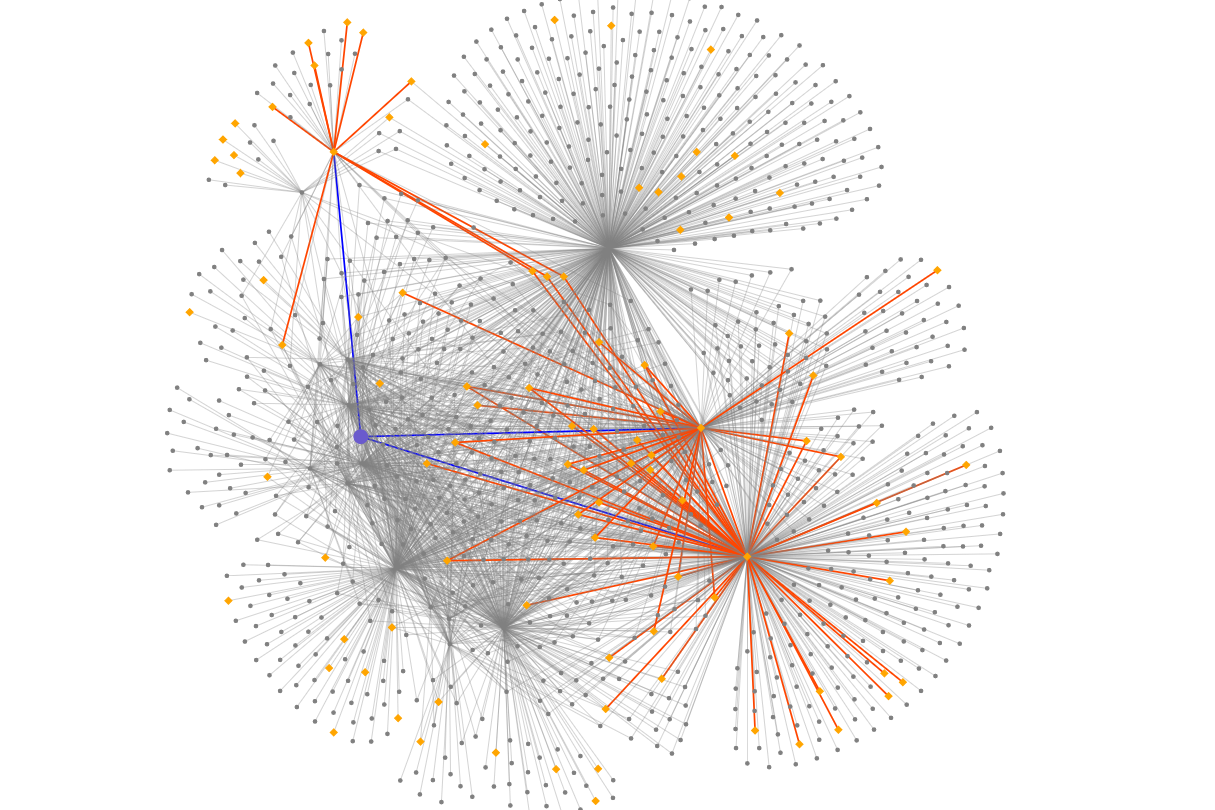
\includegraphics[width=0.8\linewidth]{images/plots/hyperreflexia_NO_SON.png}
    \caption{Hyperreflexia disease pathway within the SON community. Blue edges highlights the interaction between the SON gene and the genes inside the pathway.}
    \label{fig:hyperreflexia_NO_SON}
\end{figure}

\subsection{Final considerations}\label{subsec:final_considerations}
For most of us this has been the first approach to bioinformatics, as such we faced many difficulties, especially in the absence of a uniform notation for the data, in the different ways each database uses to represent the knowledge. 
\vspace{3mm}

Difficulties can also be challenging, after the first, quite annoying, phase of data preparation, the following steps towards the pathway analysis were way more interesting, particularly getting in touch with real world problems and their incredible complexity. Working at something that could (in potential) be lifechanging for someone has a total different feedback and has given us much more motivation than many other works.
\vspace{3mm}

Putting aside all the difficulties, we were able to achieve what was requested and possibly discovering other diseases that might be correlated to the SON gene as shown in \autoref{subsec:diseases_no_son}, so we can say that our month-long work was useful.

\appendix
\section{How to run the project}\label{sec:run_project}
The project is hosted on a github repository, so to work with there is just need to clone it.
\begin{minted}[fontsize=\small, breaklines]{bash}
git clone https://github.com/nikodallanoce/ComputationalHealthLaboratory
\end{minted}
Then, create a new python or conda environment (higly recommended) or install the required packages under an already existing environment.
\begin{minted}[fontsize=\small, breaklines]{bash}
pip install -r requirements.txt
\end{minted}
After that you can run the the jupyter notebooks, which follow the roadmap explained in \autoref{subsec:project_roadmap}:
\begin{itemize}
    \item \textbf{0\_Pathway\_Enrichment.ipynb}, deals with \autoref{sec:geneset_expansion} and \autoref{sec:pathway_enrichment}.
    \item \textbf{1\_Network\_Analysis.ipynb}, deals with \autoref{sec:network_analysis}.
    \item \textbf{2\_Community\_Analysis.ipynb}, deals with \autoref{sec:community_analysis}.
    \item \textbf{3\_Plots.ipynb}, methods to plot the protein, disease and community graphs.
    \item \textbf{4\_Project\_CHL.ipynb}, all the previous notebooks above combined.
\end{itemize}
It is also extremely important to modify the \textit{config.yml} with a valid token to access the BioGRID \cite{biogrid} datasets. You can also check the source methods inside the \textit{src} directory to have a better look on our work.
\section*{References}
%From where you are taking information, where a reader can find details, credits, sources \dots See any paper bibliography to take examples. The items here should be numbered and the number should be used in the text. \textbf{Double check the bibliography}!!! \\ \\
%In particular, always include (with a uniform style): \\

%Authors, Title, Journal/Proceedings/Editor, Volume, Pages, Year (URL if needed) \\ %\\
%E.g.: 
%\bibliographystyle{plain}
\setcitestyle{square}
\bibliographystyle{plain}
\thispagestyle{empty}
\vspace{-1cm}\bibliography{references}
\end{document}
